\documentclass[12pt]{extarticle}

\usepackage{amsmath}
\usepackage{unicode-math}
\usepackage{xltxtra}
\usepackage{xgreek}

\setmainfont{Liberation Serif}

\usepackage{tabularx}

\pagestyle{empty}

\usepackage{geometry}
\geometry{a4paper, total={190mm,275mm}, left=10mm, top=10mm}

\usepackage{graphicx}
\graphicspath{ {images/} }

\usepackage{wrapfig}

\begin{document}
\renewcommand{\labelenumi}{\alph{enumi})}
\renewcommand{\labelenumii}{\roman{enumii}.}

k\begin{table}
    \small
    \begin{tabularx}{\textwidth}{ c X r }
        \begin{tabular}{ c }
            
\includegraphics[scale=0.4]{ελληνική}         \\
            ΕΛΛΗΝΙΚΗ ΔΗΜΟΚΡΑΤΙΑ                           \\
            ΥΠΟΥΡΓΕΙΟ ΠΑΙΔΕΙΑΣ \& ΘΡΗΣΚΕΥΜΑΤΩΝ            \\
            ΠΕΡΙΦΕΡΕΙΑΚΗ Δ/ΝΣΗ Α/ΘΜΙΑΣ \& Β/ΘΜΙΑΣ ΕΚΠ/ΣΗΣ \\
            ΚΕΝΤΡΙΚΗΣ ΜΑΚΕΔΟΝΙΑΣ                          \\
            Δ/ΝΣΗ Β/ΘΜΙΑΣ ΕΚΠ/ΣΗΣ ΑΝ. ΘΕΣ/ΝΙΚΗΣ           \\
            10ο ΓΕΝΙΚΟ ΛΥΚΕΙΟ ΘΕΣ/ΝΙΚΗΣ
        \end{tabular}
         &  &
        \begin{tabular}{ r }
            Σχολικό Έτος: 2022 - 2023     \\
            Εξ. Περίοδος: Μαΐου - Ιουνίου \\
            Μάθημα: Γεωμετρία Β Λυκείου   \\
            Εισηγητής: Λόλας              \\ \\
            Θεσσαλονίκη, 26 / 05 / 2023
        \end{tabular}
    \end{tabularx}
\end{table}

\part*{\centering{Θέματα}}
\section*{Θέμα 1}
\noindent

\begin{enumerate}
    \item Να αποδείξετε ότι το εμβαδόν Ε ενός τριγώνου είναι ίσο με το ημιγινόμενο μιας πλευράς επί το αντίστοιχο ύψος. \hspace*{\fill} \textbf{Μονάδες 15}

    \item Να χαρακτηρίσετε τις παρακάτω προτάσεις με Σωστό ή Λάθος
          \begin{enumerate}
              \item Το τετράγωνο της κάθετης πλευράς ενός ορθογωνίου τριγώνου ισούται με το γινόμενο της κάθετης πλευράς με την υποτείνουσα.
              \item Το μήκος ενός τόξου $α$ ακτινίων σε κύκλο ακτίνας $R$ είναι $l=αR$.
              \item Ο λόγος ομοιότητας των εμβαδών δύο όμοιων σχημάτων ισούται με τον λόγο ομοιότητας των πλευρών του.
              \item Κανονικό πολύγωνο είναι το σχήμα που έχει όλες τις πλευρές του ίσες.
              \item Σε τρίγωνο με πλευρές $α$, $β$, $γ$, αν ισχύει $β^2<α^2+γ^2$ τότε $\hat{Β}<90^{\circ}$.\hspace*{\fill}\textbf{Μονάδες 10}
          \end{enumerate}
\end{enumerate}

\section*{Θέμα 2 (21350)}
\noindent
Στο σχήμα δίνονται ότι $\hat{Β}=\hat{Ε}=90^{\circ}$, $ΑΕ=8$, $ΕΒ=4$ και $ΔΕ=4$.
\begin{enumerate}
    \item[α)] Να αποδείξετε ότι τα τρίγωνα $ΑΕΔ$ και $ΑΒΓ$ είναι όμοια \hspace*{\fill} \textbf{Μονάδες 10}
    \item[β)] Να γράψετε τους ίσους λόγους που προκύπτουν από την ομοιότητα των τριγώνων $ΑΕΔ$ και $ΑΒΓ$

        \hspace*{\fill} \textbf{Μονάδες 10}
    \item[γ)] Να υπολογίσετε το μήκος της πλευράς $ΒΓ$ \hspace*{\fill} \textbf{Μονάδες 5}
\end{enumerate}
\begin{figure}[h]

    \centering
    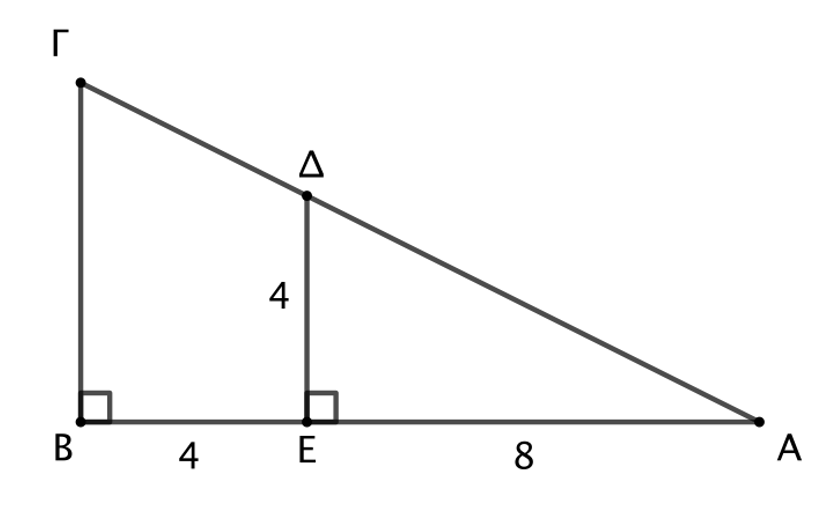
\includegraphics[width=0.50\textwidth]{2023(2)}
\end{figure}

\section*{Θέμα 3}
\noindent

\begin{wrapfigure}[3]{r}{0.38\textwidth}
    \centering
    \vspace{-20pt}
    \hspace{-80pt}
    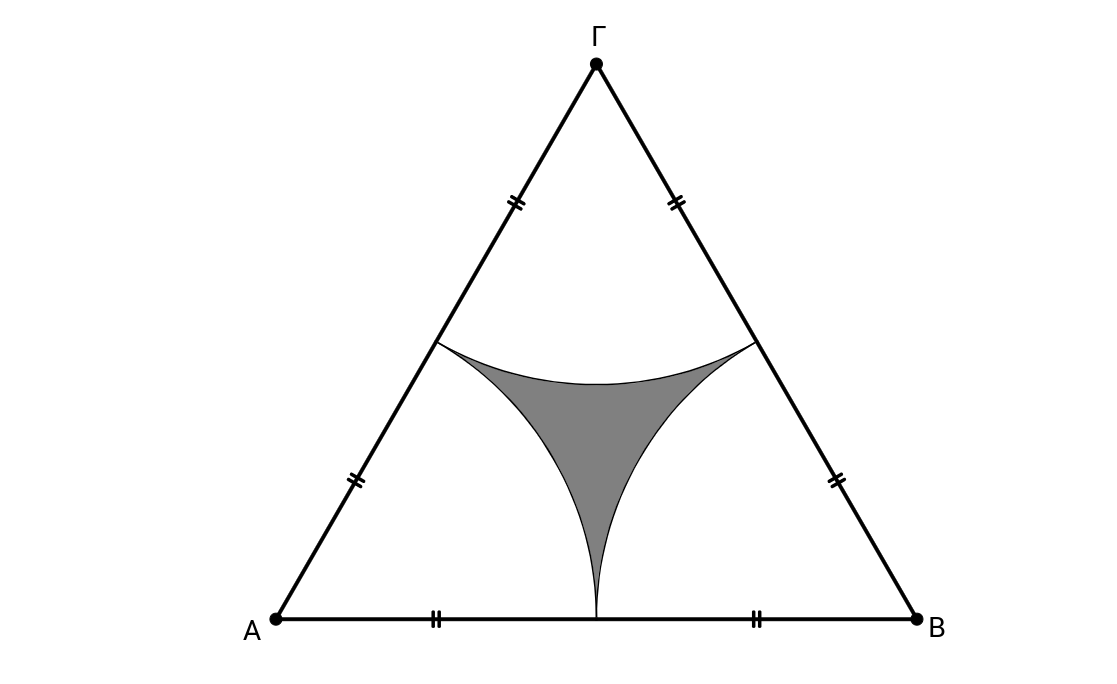
\includegraphics[width=0.38\textwidth]{2017BGeo3}
\end{wrapfigure}

Έστω ισόπλευρο τρίγωνο πλευράς $2R$. Με κέντρο κάθε κορυφή εγγράφουμε στο τρίγωνο κυκλικούς τομείς ακτίνας $R$ όπως το διπλανό σχήμα.
\begin{enumerate}
    \item[α)] Να βρείτε την περίμετρο του γραμμοσκιασμένου σχήματος ως προς $R$. \hspace*{\fill} \textbf{Μονάδες 9}
    \item[β)] Να δείξετε ότι το ύψος του τριγώνου είναι $R\sqrt{3}$. \hspace*{\fill} \textbf{Μονάδες 4}
    \item[γ)] Να δείξετε ότι το εμβαδό του τριγώνου είναι $R^2\sqrt{3}$. \hspace*{\fill} \textbf{Μονάδες 3}
    \item[δ)] Να υπολογίσετε το εμβαδό του γραμμοσκιασμένου τμήματος ως προς $R$. \hspace*{\fill} \textbf{Μονάδες 9}
\end{enumerate}

\section*{Θέμα 4 (16135)}
\noindent

Δίνεται το τρίγωνο $ΑΒΓ$ με υποτείνουσα $ΒΓ=10$ και έστω ότι $Δ$ είναι η προβολή της κορυφής $Α$ στην $ΒΓ$.
\begin{enumerate}
    \item[α)] Αν $ΔΒ=2$ να υπολογίσετε
        \begin{enumerate}
            \item το ύψος $ΑΔ$ του τριγώνου $ΑΒΓ$ \hspace*{\fill} \textbf{Μονάδες 7}
            \item το εμβαδόν του τριγώνου $ΑΒΓ$ \hspace*{\fill} \textbf{Μονάδες 5}
        \end{enumerate}

    \item[β)] Υποθέστε ότι το σημείο $Α$ κινείται πάνω στο ημικύκλιο με διάμετρο την $ΒΓ$
        \begin{enumerate}
            \item Να ποδείξετε ότι το εμβαδόν του τριγώνου $ΑΒΓ$ είναι $(ΑΒΓ)=5ΑΔ$ \hspace*{\fill} \textbf{Μονάδες 7}
            \item Θεωρήστε τον παρακάτω ισχυρισμό:

                  "Για όλες τις θέσεις του $Α$ πάνω στο ημικύκλιο με διάμετρο την $ΒΓ$, το εμβαδόν του τριγώνου $ΑΒΓ$ δεν υπερβαίνει το 25"

                  Είναι αληθής ή ψευδής ο παραπάνω ισχυρισμός; Να αιτιολογήσετε την απάντησή σας. \hspace*{\fill} \textbf{Μονάδες 6}
        \end{enumerate}
\end{enumerate}
\begin{figure}[h]

    \centering
    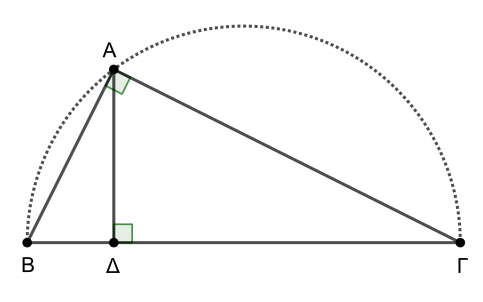
\includegraphics[width=0.50\textwidth]{2023(4)}
\end{figure}

\begin{table}[htb]
    \begin{tabularx}{\textwidth}{ X c X c X}
         &
        \begin{tabular}[t]{ c }
            Ο Δ/ντης \\ \\ \\ \\
            Παπαδημητρίου Χρήστος
        \end{tabular}
         &   &
        \begin{tabular}[t]{ c }
            Ο εισηγητής \\ \\ \\ \\
            Λόλας Κωνσταντίνος
        \end{tabular}
         &
    \end{tabularx}
\end{table}
\end{document}